%#!platex -src-specials CategoryTheory.tex
\chapter{抽象的な構造}\label{Ch:Abstract Structure}
この章では,圏論\index{けんろん@圏論}的定義についての幾つかの注意喚起か
ら始めたい.圏論的定義とは圏論的な言葉,つまり他の対象や射との
関係のみによる性質の特徴付けである.そうした定義の仕方は,構造的であると
か,操作的,関係的,あるいはもしかしたら(内部的と対比して)外部的な定義
であると呼ばれたりする.対象や射は,それらが圏の中で他とどう関係するかと
いう役割のみによって,つまり構造\index{こうそう@構造}の中での位置関係の
みによって決まるのであって,それらが「何であるか」「何でできているか」に
ついては全く関係ないとするのがこの考え方である.以前に見た自由圏
や自由モノイド,あるいは圏の構築といったものがそうした定義の例である.ま
た,今後さらに多くの例を見ていく.以下では,とても単純な例から始める.我々
はこれを{\bfseries 抽象的な特徴付け}と呼ぼう.そうした特徴付けを行なう基
本的な方法は,普遍写像性\index{ふへんしやそうせい@普遍写像性}を通しての
ものである,ということがわかるだろう.

\section{エピとモノ}
$\Sets$において,写像$f: A\to B$は,
\begin{quotation}
 任意の$a, a' \in A$ に対し $f(a) = f(a')$ ならば $a = a'$ が成立すると
 き{\bfseries 単射}\index{しやそう@写像!たんしや@単射---}

 任意の$b \in B$ に対しある $a \in A$ があって $f(a) = b$ が成立するとき
 {\bfseries 全射}\index{しやそう@写像!せんしや@全射---}
\end{quotation}
であるとそれぞれ呼ばれたことを思い出そう.これらの性質に対する抽象的特徴付けは,
次の通りである.

\begin{definition}
 任意の圏 ${\bf C}$ において,射$f: A \to B$が

 \begin{quotation}
  {\bfseries モノ射}\index{ものしや@モノ射}
  \index{もの@モノ|see{モノ射}}であるとは,任意の射 $g, h: C \to A$ につ
  いて $fg = fh$ ならば$g = h$が,
  \begin{center}
   \begin{tikzpicture}
    \matrix (m) [matrix of math nodes, column sep=2cm] { C & A & B \\};
    \path[->]
      (m-1-1.20) edge node {$g$} (m-1-2.160)
      (m-1-1.340) edge node [swap]{$h$} (m-1-2.200)
      (m-1-2) edge node {$f$} (m-1-3);
   \end{tikzpicture}
  \end{center}

  {\bfseries エピ射}\index{えひしや@エピ射}
  \index{えひ@エピ|see{エピ射}}であるとは,任意の射 $i, j: B \to D$ につ
  いて $if = jf$ ならば $i = j$が,
  \begin{center}
   \begin{tikzpicture}
    \matrix (m) [matrix of math nodes, column sep=2cm] { A & B & D \\};
    \path[->]
      (m-1-2.20) edge node {$i$} (m-1-3.160)
      (m-1-2.340) edge node [swap]{$j$} (m-1-3.200)
      (m-1-1) edge node {$f$} (m-1-2);
   \end{tikzpicture}
  \end{center}
 \end{quotation}
 それぞれ成り立つことである.しばしば,$f$がモノ射のとき
 $f: A \mono B$と書き,$f$がエピ射のとき $f: A \epi B$ とかく
 \footnote{訳注:「モノである」ことを「モニック(monic)」,「エピである」
 ことを「エピック(epic)」という.}.
\end{definition}
\begin{prop}
 集合の間の写像$f: A \to B$ は,$f$が単射であるとき,その時に限りモノ射
 となる.
\end{prop}

\begin{proof}[証明]
$f: A \mono B$ とする.$a, a' \in A$ について $a \neq a'$として,
 $\{x\}$を適当な一点集合とする.ここで,
 \[
  \bar a(x) = a,\, \bar{a'}(x) = a'
 \]
 で定義される写像
 \[
  \bar a, \bar{a'}: 1 \to A
 \]
 を考える.今,$f$はモノ射なので,$\bar a \neq \bar{a'}$ より
 $f\bar a \neq f\bar{a'}$ である.従って,
 $f(a) = (f\bar a)(x) \neq (f\bar{a'})(x) = f(a')$となるので,$f$は単射
 である.

 逆に,$f$を単射とし,写像$g, h:C \to A$ について$g \neq h$,つまりある
 $c \in C$について $g(c) \neq h(c)$ とする.$f$は単射なので,
 $f(g(c)) \neq f(h(c))$となり,従って $fg \neq fh$となる.
\end{proof}

\begin{example}\label{monos and injs}
 モノイドなどの「構造の入った集合」
 \index{しゆうこう@集合!こうそうのはいつた@構造の入った---}
 からなる圏の多くでは,モノ射と「単射準同型」の概念は一致する.より精確
 にいえば,モノイド準同型$h: M \to N$ はその台写像 $|h|: |M| \to |N|$ が
 モノ射であるときに限りモノ射となり,従って前の議論より単射となる.これを証
 明するため,$h$をモノとし,二つの異なる「元」$x, y: 1 \to |M|$ を取ろう
 (但し,$1 = \{*\}$なる一点集合とする).自由モノイド$M(1)$の普遍写像性より対
 応する準同型$\bar x, \bar y: M(1) \to M$が存在する.また,$h$はモノ射な
 ので,その合成射 $h \circ \bar x, h \circ \bar y: M(1) \to M \to N$は異
 なる射となる.従って,再び$M(1)$の普遍写像性より対応する「元」
 $hx, hy: 1 \to N$ もまた異なる.
 \begin{center}
  \begin{tikzpicture}
    \matrix (m) [matrix of math nodes, column sep=2cm, row sep=2cm] {
     M(1) & M & N \\
     1 & \left|M\right| & \left|N\right|\\};
    \path[->]
      (m-1-1.10) edge node {$\bar x$} (m-1-2.165)
      (m-1-1.350) edge node [swap]{$\bar y$} (m-1-2.200)
      (m-1-2) edge node {$h$} (m-1-3)
      (m-2-1.20) edge node {$x$} (m-2-2.165)
      (m-2-1.340) edge node [swap]{$y$} (m-2-2.190)
      (m-2-2) edge node {$|h|$} (m-2-3);
  \end{tikzpicture}
 \end{center}

 逆に,$|h|: |M| \to |N|$がモノ射で,$f, g: X \to M$ が任意の異なる準同
 型であるとする.このとき,$|f|, |g|: |X| \to |M|$ は異なる写像であり,
 $|h|$がモノ射であるので$|h| \circ |f|, |h| \circ |g|: |M| \to |N|$ も同
 様に異なる.$|h \circ f| = |h| \circ |f| \neq |h| \circ |g| = |h \circ g|$
 であるので,従って$h\circ f \neq h\circ g$でなくてはならない.
\end{example}
全く同じ状況が群や環\index{かん@環},ベクトル空間
\index{へくとるくうかん@ベクトル空間},poset などでも成立する.この事実
は,こうした対象からなる圏に自由モノイド$M(1)$に相当する対象が存在する
ことから従う.

\begin{example}\label{poset and mono/epi}
 poset ${\bf P}$において,任意の射 $p \leq q$はモノかつエピとなる.
 何故か?
\end{example}

さて,今迄のと双対的に,$\Sets$のエピ射は全射写像と一致する(演習問題!).
しかしそれとは対照的に,以下で見るように他のよく知られた圏ではエピ射が単
に全射準同型であるとは限らない.

\begin{example}\label{monoid and epis}
 モノイドとその準同型からなる圏$\Mon$において,モニックな準同型
 \[
  h: \N \mono \Z
 \]
 が存在する.ここで,$\N$は自然数の加法モノイド$(N, +, 0)$,$\Z$は整数の
 加法モノイド$(Z, +, 0)$ である.この,集合の埋め込み$\N \subseteq \Z$で
 得られる対応が, $\Mon$ においてはエピ射でもある 
 \index{えひしや@エピ射!ものいとの@モノイドの---}ことを,次の事実を示す
 ことで証明しよう:

 任意のモノイド準同型 $f,g: (\Z, +, 0) \to (M, *, u)$ が与えられた時,そ
 の $N$ への制限が一致するとき,即ち $f|_N = g|_N$ となるとき $f=g$とな
 る.

 まず始めに注意することは,
 \begin{align*}
  f(-n) &= f((-1)_1 + (-1)_2 + \cdots + (-1)_n)\\
        &= f(-1)_1 * f(-1)_2 * \cdots * (-1)_n
 \end{align*}
 が成立し,$g$に関しても同様の事実が成立することである.したがって,上の
 議論は $f(-1) = g(-1)$を示すことに帰着される.しかるに,
 \begin{align*}
  f(-1) &= f(-1) * u\\
        &= f(-1) * g(0)\\
        &= f(-1) * g(1-1)\\
        &= f(-1) * g(1) * g(-1)\\
        &= f(-1) * f(1) * g(-1)\\
        &= f(-1 + 1) * g(-1) \\
        &= f(0) * g(-1)\\
        &= u * g(-1)\\
        &= g(-1)
 \end{align*}
 よって示された.
\end{example}

注意すべきなのは,代数的観点からは,射$e$がエピ射であるのは右側の$e$が簡
約出来るとき,つまり $xe = ye$ ならば $x = y$ が成立するときのみであり,
$m$ がモノ射であるのも$m$が左簡約可能であるとき,つまり$mx = my$ ならば
$x = y$が成立するときに限られるということである.

\begin{prop}
 任意の同型射\index{とうけいしや@同型射}はモニックかつエピックである.
\end{prop}
\begin{proof}[証明]
 次の図式を考える.
 \begin{center}
  \begin{tikzpicture}
   \matrix (m) [matrix of math nodes, column sep=2cm, row sep=2cm] {
   A & B & C\\
     &   & B & D\\
   };

   \path[->]
     (m-1-1.20) edge node {$x$} (m-1-2.160)
     (m-1-1.340) edge node [swap]{$y$} (m-1-2.200)
     (m-1-2) edge node {$m$} (m-1-3)
             edge node {$1$} (m-2-3)
     (m-1-3) edge node {$e$} (m-2-3)
     (m-2-3.20) edge node {}(m-2-4.160)
     (m-2-3.340) edge node {} (m-2-4.200);
  \end{tikzpicture}
 \end{center}

 もし$m$ が $e$ を逆射とする同型射なら,$mx = my$ ならば
 $x = emx = emy = y$が成立し,従って$m$はモノ射となる.同様にして, $e$
 は右簡約可能となり,従ってエピ射となる.
\end{proof}
$\Sets$においては上の逆が成立する.つまり,モニックかつエピックな射は
同型射となる.しかし,モノイドの例からもわかるとおり,これは一般には成立
しない.

\subsection{断面と引き込み}
\index{たんめん@断面|(}
\index{せくしよん@セクション|see{断面}}
\index{ひきこみ@引き込み|(}
\index{れとらくしよん@レトラクション|see{引き込み}}
どんな同型射もモニックかつエピックであることは既に見た.より一般に,射
\[
 f: A \to B
\]
が左逆射
\[
 g: B \to A,\;\;gf = 1_A
\]
を持てば,同様の議論により$f$はモノ射,$g$はエピ射でなければならない.

\begin{definition}
 {\bfseries 分裂}({\itshape split})モノ射(エピ射)
 \index{えひしや@エピ射!ふんれつ@分裂---}
 \index{ものしや@モノ射!ふんれつ@分裂---}とは,左(右)逆射を持つ射のこ
 とである.射$e:X \to A$ と$s: A \to X$ があって$es = 1_A$ を満たすとき,
 射 $s$ は $e$ の{\bfseries 断面}({\bfseries セクション};{\itshape
 section})% \index{たんめん@断面|textit}
 または{\bfseries 分裂}({\itshape splitting})と呼ばれ,
 $e$ は$s$の{\bfseries 引き込み}({\bfseries レトラクション};{\itshape
 retraction}) % \index{ひきこみ@引き込み|textit}
 と呼ばれる.このとき,対象 $A$ は $X$ の{\bfseries レトラ
 クト}({\itshape retract})\index{れとらくと@レトラクト|textit}と呼ばれ
 る.
\end{definition}

函手\index{かんしゆ@函手}は恒等射を保つので{\bfseries 分裂}エピ射と
{\bfseries 分裂}モノ射も保存される.上の例$\ref{monoid and epis}$でやっ
たように $\Mon$ の忘却函手
\[
 \Mon \to \Sets
\]
はエピ射$\N \to \Z$を保存しないことと比較せよ.

\begin{example}\label{splits and AC}
 $\Sets$では,
 \[
  \emptyset \mono A
 \]
 の形を除く任意のモノ射は分裂する.{\bfseries 任意のエピ射は分裂射である}と
 いう条件は,選択公理の圏論的表現になっている.エピ射
 \[
  e: E \epi X
 \]
 について考えよう.この時,空でない集合の族
 \[
  E_x = e^{-1}\{x\},\;\; x \in X
 \]
 が存在する.この族$(E_x)_{x \in X}$に対する選択函数
 \index{かんすう@函数!せんたく@選択---}は,正に$e$の断面,すなわち
 $es = 1_X$ なる$s: X \to E$である.何故なら,任意の $x \in X$ に対し,
 $s(x) \in E_x$ となるからである.

 逆に,非空集合の族
 \[
  (E_x)_{x\in X}
 \]
 に対し,$E = \set{(x, y) | x \in X, y \in E_x}$ とし,エピ射
 $e: E \epi X$を$(x, y) \mapsto x$で定める.すると,$e$の断面$s$は明らか
 に族に対する選択函数を決定している.
\end{example}

「対象の族」\index{たいしよう@対象!のそく@---の族}はある一つの射 $e: E \to X$
の「ファイバー」によって表現出来る.この考え方は上での議論より広い応用を
持っており,7.10で詳しく検討する.

「選択函数」\index{かんすう@函数!せんたく@選択---}の存在に関連する概念のひ
とつに「射影的」の概念がある.対象$P$が{\bfseries 射影的}({\itshape projective})
\index{たいしよう@対象!しやえいてき@射影的---}であるとは,任意のエピ射
$e: E \epi X$ と射 $f: P \to X$について,ある(一意とは限らない)射
$\bar f: P \to E$ があって,次の図式のように$e \circ \bar f = f$となるこ
とである.
\begin{center}
 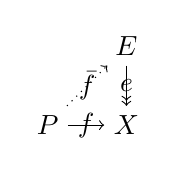
\begin{tikzpicture}
  \node (E) {$E$};
  \node (X) [below of=E] {$X$};
  \node (P) [left of=X] {$P$};

  \path[->>] (E) edge node [swap]{$e$} (X);
  \path[->, dotted] (P) edge node {$\bar f$} (E);
  \path[->] (P) edge node [swap] {$f$} (X);
 \end{tikzpicture}
\end{center}
この状況を,$f$は$e$を{\bfseries 持ち上がる}\index{もちあかる@持ち上がる}
($f$ {\itshape lifts across} $e$)などということがある.射影的対象へのエピ
射は明らかに分裂射である.射影的対象はより「自由」な構造を持つと考えるこ
とができ,従って「より多くの射」を許容する.

選択公理は任意の集合が射影的であることを主張しており,そのことから代数系から
なる圏の多く(全てではない!)では,自由対象もまた射影的であることがいえ
る.また,任意の圏において,射影的対象のレトラクトが再び射影的となること
を読者は確かめるべきである.
\index{たんめん@断面|)}
\index{ひきこみ@引き込み|)}
\section{始対象と終対象}
\label{Ch:initial and terminal objects}
それでは,圏$\Sets$の空集合や一点集合,および一般の圏における似た構造を
持った対象の抽象的特徴付けを見ていこう.

\begin{definition}
 任意の圏${\bf C}$において,
 
 対象$0$が{\bfseries 始対象}であるとは,どんな対象$C$についても,それをコド
 メインに持つ射が一意に存在することである.
 \index{たいしよう@対象!し@始---|(}
 \index{ふへんしやそうせい@普遍写像性!したいしようの@始対象の---}
 \begin{center}
  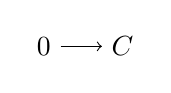
\begin{tikzpicture}
   \node (0) {$0$};
   \node (C) [right of=0]{$C$};
   \draw[->] (0) to (C);
  \end{tikzpicture} 
 \end{center} 

 対象$1$が{\bfseries 終対象}であるとは,どんな対象$C$についても,それをド
 メインに持つ射が一意に存在することである.
 \index{たいしよう@対象!しゆう@終---|(}
 \index{ふへんしやそうせい@普遍写像性!しゆうたいしようの@終対象の---}
 \begin{center}
  \begin{tikzpicture}
   \node (1) {$1$};
   \node (C) [left of=0]{$C$};
   \draw[->] (C) to (1);
  \end{tikzpicture} 
 \end{center} 
\end{definition}

モノ射やエピ射の場合と同様,この定義においても或る種の「双対性」が成立し
ていることに注意しよう.精確にいえば,${\bf C}$での終対象は正に
${\bf C}^{\rm op}$での始対象になっているのである.この双対性については,
第\ref{Ch:Duality}章で体系的に考察する.

まず手始めに,始対象や終対象の概念は単純な普遍写像性によって定義されるた
め,自由モノイドと同様に同型を除いて一意に決定されることを見よう.

\begin{prop}
 始対象(終対象)は,(存在すれば)同型を除いて一意である.
\end{prop}
\begin{proof}
 事実,もし$C$と$C'$が共に同じ圏の始対象(終対象)であれば,同型射
 $C\to C'$が{\bfseries 一意}に存在する.実際,$0$と$0'$をある圏
 ${\bf C}$の始対象とする.すると,次の図式より,$0$ と $0'$は明らかに一
 意的に同型となることがわかる.
 \begin{center}
  \begin{tikzpicture}
   \matrix (m) [matrix of math nodes, column sep=2cm, row sep=2cm] {
    0 & 0'\\
      & 0 &  0'\\
   };
   \path[->]
     (m-1-1) edge node {$u$} (m-1-2)
             edge node [swap]{$1_0$} (m-2-2)
     (m-1-2) edge node {$v$} (m-2-2)
             edge node {$1_{0'}$} (m-2-3)
     (m-2-2) edge node [swap]{$u$} (m-2-3);
  \end{tikzpicture}
 \end{center}
 終対象に関しては,上の議論を ${\bf C}^{\rm op}$に適用すればよい.
\end{proof}

\begin{example} 

 \begin{enumerate}
  \item $\Sets$ においては,空集合が始対象であり,任意の一元集合 $\{x\}$
	が終対象となる.$\Sets$は唯一つの始対象をもつのに対し,終対象は
	無数に存在することに注目しよう(これは$\Sets \cong \Sets^{\rm
	op}$が成立するか,という問いの答えを与えている).
  \item $\Cat$\index{Cat@$\Cat$}では,圏${\bf 0}$(対象も射も持たない)
	が始対象,圏${\bf	1}$(ひとつの対象とその恒等射を持つ)が
	終対象となる.
  \item ${\bf Groups}$では,単位群が始対象{\bfseries かつ}終対象となっ
	ている(ベクトル空間と線形変換からなる圏や,モノイドとモノイド準
	同型からなる圏も同様である).しかし,${\bf Rings}$(単位元を持
	つ可換環\index{かん@環}からなる圏)では,整数全体$\Z$が始対象と
	なる($0 = 1$とした一元環が終対象である).
  \item {\bfseries ブール代数}\index{ふーるたいすう@ブール代数}とは,特
	別な元 $0, 1$と,「結び(join)」$a \vee b$,「交わり(meet)」
	$a \wedge b$と呼ばれる二項演算,および「補元」を取る単項演算
	$\neg b$を持つ poset \index{poset}$B$ のことである.これらの演算
	は次の条件を満たさなくてはならない.
	\begin{eqnarray*}
	 &0 \leq a&\\
	 &a \leq 1&\\
	 a \leq c \text{かつ} b \leq c &\iff& a \vee b \leq c\\
	 c \leq a \text{かつ} c \leq b &\iff& c \leq a \wedge b\\
	 a \leq \neg b  &\iff& a \wedge b = 0\\
	 &\neg \neg a = a&
	\end{eqnarray*}
	順序を用いずに等式関係のみを用いた同値な特徴付けもある.

	ブール代数の典型的な例として,集合$X$の部分集合全体からなる冪集
	合\index{しゆうこう@集合!へき@冪---}$\Pow(X)$
	に包含関係$A \subseteq B$ を入れたものがある.この時のブール演算
	は,空集合 $0 = \emptyset$,全体集合 $1 = X$として,和集合および
	共通部分を結びおよび交わり,相対補集合$X - A$を$\neg A$とする.
	よく知られた特別な場合として,二元ブール代数${\bf 2} = \{0, 1\}$
	(冪集合 $\Pow(1)$と見ることができる)があり,選言(論理和),連
	言(論理積),否定などの論理演算をブール演算として元を「真理値」
	と見做すことがある.これは,ブール代数の圏${\bf BA}$の始対象とな
	る.${\bf BA}$は射としてブール準同型を持つ.すなわち,函手
	$h: B \to B'$は$h(0) = 0,\, h(a \vee b) = h(a) \vee h(b)$ など
	追加的な構造を保つ.一元ブール代数(即ち$\Pow(0)$)が終対象とな
	る.
  \item poset では,始対象となるのは明らかに最小元のみであり,終対象も最
	大元のみである.したがって,例えば任意のブール代数は始対象と終対
	象の両方を持つ.明らかに,圏だからといって両方ともを持つ
	{\bfseries 必要はない}.例として,poset $(\Z, \leq)$には始対象も
	終対象も存在しない.
  \item 任意の圏${\bf C}$と対象$X \in {\bf C}$について,恒等射
	$1_X: X	\to X$はスライス圏${\bf C}/X$の終対象であり,コスライス
	圏$X/{\bf C}$の始対象である.
 \end{enumerate}
\end{example}
\index{たいしよう@対象!し@始---|)}

\section{一般化元}
\index{けん@元!いつはんか@一般化---|(}
終対象および始対象に出入りする射について考察しよう.興味の対象となるのは
明らかにその内でも限られたものだけだが,それらはとても重要となる.

集合 $A$ が始対象への射 $A \to 0$を持つのは$A$がそれ自身始対象であるとき
だけであり,posetについても同様のことがいえる.それに対して,モノイドや
群については,始対象と終対象は一致するので,全ての対象は始対象へ
の射を唯一つだけ持つ.

しかし,ブール代数\index{ふーるたいすう@ブール代数}の圏 ${\bf BA}$では状
況は完全に異なる.始ブール代数${\bf 2}$へのマップ$p: B \to {\bf 2}$は,
$B$の{\bfseries ウルトラフィルター}({\itshape ultrafilter})$U$
\index{うるとらふいるたー@ウルトラフィルター}
\index{ふいるたー@フィルター!うるとら@ウルトラ---|see{ウルトラフィルター}}
と呼ばれるものと一意に対応する.ブール代数$B$の{\bfseries フィル
ター}({\itshape filter})\index{ふいるたー@フィルター}とは,空でない部
分集合$F \subseteq B$であって交わりについて上に閉じているものである:
\begin{align*}
 a \in F \text{かつ} a \leq b\  &\text{ならば} \ b \in F\\
 a \in F \text{かつ} b \in F\  &\text{ならば} \ a \wedge b \in F
\end{align*}
$F$を含むフィルター$F \subset F'$が「真でない」,即ち$B$全体に限られる
とき,$F$は{\bfseries 極大}({\itshape maximal})であるといわれる.
{\bfseries ウルトラフィルター}とは,極大フィルター
\index{ふいるたー@フィルター!きよくだい@極大---}の
ことである.フィルター$F$は,任意の元 $b \in B$に対し$b \in F$か
$\neg b \in F$のどちらか一方のみが成立するとき,その時に限ってウルトラフィ
ルターとなる.このことを示すのはさして難しいことではない(演習問題!).
さて,$p: B \to {\bf 2}$としたとき,$U_p = p^{-1}(1)$によってウルトラフィ
ルター $U_p \subset B$を定めよう.また,ウルトラフィルター$U \subset B$
が与えられた時,$b \in U$ならばその時に限って$p_U(b) = 1$として,ブール
準同型 $p_U: B \to {\bf 2}$を定めよう.こうした操作が互いに逆演算となっ
ている事実から,これは容易に確かめることが出来る.ブール準同型
$p: B \to {\bf 2}$は,論理学において「真理表」を形成するのにも用いられる.
実際,真理表の各列は,論理式からなるブール代数上のそのような準同型と対応
している.

環準同型$A \to \Z$ は,代数幾何において上と同様かつ同じくらい重要な役割
を担っている.そうした準同型は,ウルトラフィルターの環論的な一般化である
{\bfseries 素イデアル}の概念に対応している.

さて,では終対象からの射について考えよう.$X$を任意の集合とする.任意の
$x \in X$に対し,対応する終対象$1 = \{\ast\}$からの射$\bar x:1 \to X$を
$\bar x(\ast) = x$によって定める.これにより,同型
\[
 X \cong \Hom_{\Sets}(1, X)
\]
を得る.この対応は既に何度か使っているものである.似た状況は poset(ある
いは位相空間)からなる圏でも成立する.つまり,射$1 \to P$は,poset(また
は空間)の台集合の元に対応するのである.終対象 $1$ を持つ任意の圏
${\bf C}$について,そうした射$1 \to A$は,しばしば$A$の
{\bfseries 大域元}\index{けん@元!たいいき@大域---}
({\itshape global elements}),{\bfseries 点}\index{てん@点}
({\itshape points)},または{\bfseries 定数}\index{ていすう@定数}
({\itshape constants})などと呼ばれることがある.集合やposet,空間の圏
において,一般の射$f:A \to B$は,$A$の各点にどう作用するかによって決定さ
れる.つまり,任意の点$a:1 \to A$に対して,$fa = ga$となるとき,二つの射
$f, g: A \to  b$は等しくなる.

しかし,注意すべきなのは,どんな場合でもこのような事が成立する訳ではない
ことである!モノイドの圏の対象$M$には幾つの点が存在するだろうか?つまり,
あるモノイド$M$が与えられたとき,$1 \to M$の形の射は幾つあるだろうか?一
つだけだ!では,ブール代数には幾つの点があるだろうか?

一般的に対象はその点によって決定される訳ではないので,{\bfseries 一般化
元}({\itshape generalized elements})という道具立てを導入すると便利であ
る.それは,(任意のドメイン$X$を持つ)任意の射
\[
 x: X \to A
\]
である.これらは,{\bfseries 一般化元}あるいは{\bfseries 可変元}
\index{けん@元!かへん@可変---}({\itshape variable elements})などと呼ば
れる.計算機科学\index{けいさんきかかく@計算機科学}や論理学
\index{ろんりかく@論理学}では,射 $1 \to A$を定数あるいは閉じた項,一般
の射$X \to A$を任意の項と見做すことが良くある.これらをまとめると次のよ
うになる.
\begin{example} 

 \begin{enumerate}
 \item $\Pos$の射$f, g:P \to Q$を考える.すると,全ての$x: 1 \to P$に対
       し$fx = gx$となるとき,その時に限り$f = g$となっている.この意味
       で,poset は射を分離するのに「十分に多くの点」
       \index{てん@点!しゆうふんにおおくの@十分に多くの---}
       を持っている.
 \item 対照的に$\Mon$では,モノイド$M$は唯一つの点しか持たないため,どん
       な準同型$h, j: M \to N$に対しても,全ての$x: 1 \to M$で$hx = jx$
       となってしまう.従って,モノイドは「十分に多くの点」を持っていない.
 \item しかし,${\bf C}$を任意の圏とすると,任意の$f, g: C \to D$に対し,
       全ての $x: X \to A$について$fx = gx$を満たすとき,その時に限り
       $f = g$が成り立つ(何故か?).従って,任意の対象は十分な一般化元
       を持つ.
 \item 事実,ある「試験」対象$T$を固定して,$T \to A$の形の一般化元だけ
       を考えれば十分であることがしばしばある.以下ではそれについて考察
       しよう.
 \end{enumerate}
\end{example}
\index{たいしよう@対象!しゆう@終---|)}
一般化元は色々な条件を「テスト」するのに役立つ.例として,次の形の図式を
考える.
\begin{center}
 \begin{tikzpicture}
  \matrix (m) [matrix of math nodes, column sep=2cm] { X & A & B \\};
  \path[->]
    (m-1-1.20)  edge node {$x$} (m-1-2.160)
    (m-1-1.340) edge node [swap] {$x'$} (m-1-2.200)
    (m-1-2) edge node {$f$} (m-1-3);
 \end{tikzpicture}
\end{center}
$f$は,任意の$x, x'$に対し$x \neq x'$なら$fx \neq fx'$が成り立つとき,モ
ニックなのであった.つまり,$f$は「一般化元について単射である」というこ
とだ.

同様に一般の圏について,図式
\begin{center}
 \begin{tikzpicture}
  \matrix (m) [matrix of math nodes, column sep=2cm, row sep=2cm] {
    A & B \\
    D & C \\
  };

  \path[->]
    (m-1-1) edge node {$f$} (m-1-2)
            edge node [swap] {$g$} (m-2-1)
    (m-1-2) edge node {$\alpha$} (m-2-2)
    (m-2-1) edge node [swap] {$\beta$} (m-2-2);
 \end{tikzpicture}
\end{center}
が可換かどうか,即ち$\alpha f = \beta g$かどうかをテストするには,全ての一
般化元$x: X \to A$ に対し,$\alpha f x = \beta g x$ が成立するかどうかを
確かめれば良い(特に$x = 1_A: A \to A$とすればよい).

\begin{example}
 一般化元は定数元よりも「更なる構造を明らかにする」のに役立てることが出
 来る.例として,次のposet $X$ と $A$ を考える.
 \begin{align*}
  X = \{x \leq y, x \leq z\}\\
  A = \{a \leq b \leq c\}
 \end{align*}
 すると,次で定義される順序を保つ全単射が存在する.
 \[
  f(x) = a,\ \ \ \  f(y) = b,\ \ \ \ f(z) = c
 \]
 $f$が圏$\Pos$でモニックかつエピックとなることを示すのは容易である.しか
 し,$f$は明らかに同型射ではない.$X$と$A$は「異なる構造
 \index{こうそう@構造}を持つ」といいた
 い人もいるだろう.そして実際,それはこれらが非同型であるということから
 出て来る.しかし,両者が(他の射$X \to A$によって)同型{\bfseries にな
 ることはない}ことを{\bfseries 証明する}にはどうすればよいだろう?一般的
 に,この種のことを示すのはとても難しい.

 二つの対象が同型でないことを示すひとつの方法は「不変量」
 \index{ふへんりよう@不変量},即ち同型射によって保存される属性を使うこと
 である.もし二つの対象が異なる不変量を持てば,それらが同型となることは
 出来ない.一般化元は不変量を定義するための簡単な手段を与える.例えば,
 $X$と$A$の大域元の個数は等しい.つまり,両者共に三つの元からなる集合で
 ある.しかし,その代わりに「試験対象」として poset ${\bf 2} = \{0 \leq 1\}$
 をとり,そこからの射「${\bf 2}$-元」${\bf 2} \to X$を考えてみよう.する
 と,$X$は${\bf 2}$-元を5つ持ち,$A$は6つ持つ.この数は不変量なので,二
 つの poset は同型にはなりえない.より詳しくいえば,任意のposet $P$に対
 して数不変量を次で定めることが出来る:
 \[
  |\Hom({\bf 2}, P)| = \Hom({\bf 2}, P)\text{の元の個数}
 \]
 すると,$P \cong Q$のとき$|\Hom({\bf 2}, P)| = |\Hom({\bf 2}, Q)|$とな
 ることは容易に示せる.何故なら任意の同型
 \begin{center}
  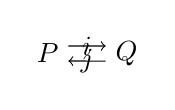
\begin{tikzpicture}
   \node (P) {$P$};
   \node (Q) [right of=P] {$Q$};

   \path[->]
     (P.20) edge node {$i$} (Q.160);
   \path[<-]
     (P.340) edge node [swap] {$j$} (Q.200);
  \end{tikzpicture}
 \end{center}
 は,任意の$f: {\bf 2} \to P,\, g:{\bf 2} \to Q$に対して$i_*, j_*$を
 \begin{align*}
  i_*(f) &= if\\
  j_*(g) &= jg
 \end{align*}
 で定めることにより,次の同型を与えるからである.
 \begin{center}
 \begin{tikzpicture}
  \matrix (m) [matrix of math nodes, column sep=2cm] {
    \Hom({\bf 2}, P) & \Hom({\bf 2}, Q)\\
  };
  \path[->] (m-1-1.5) edge node {$i_*$} (m-1-2.175);
  \path[<-] (m-1-1.355) edge node [swap] {$j_*$} (m-1-2.185);
  
 \end{tikzpicture}
 \end{center}
 じっさい,これは$\Hom(X, -)$が函手を与え,函手は同型射を保つというごく
 一般的な事実の特殊な場合になっている.
\end{example}

\begin{example}
 上の例のように,ある対象$T$の「基づく」一般化元が特に「解明的
 (revealing)」であることがよくある.そうした元を幾何学的に捉えると,
 「$A$ 内で$T$の形を取る図形」と見ることが出来る.poset の圏での射
 ${\bf 2} \to P$は,$P$で$p \leq p'$の形を取る図形である,といった具合で
 ある.例えば,既に見てきた通りモノイドの圏では終対象からの射は何の役に
 も立たないが,一つの生成元上の自由モノイド$M(1)$からの射を考えれば
 準同型を区別するのには十分である.つまり,$f, g: M \to M'$
 が等しいことを示すには,そうした$M(1)$からの射との合成が全て等しくなる
 ことを示せばよいのである.我々は$M(1) = \N$(自然数全体のモノイド)であ
 ることを知っているので,$M(1)$に基づく一般化元$M(1) \to M$は,$M$内で
 「$\N$の形をしている図形」と考えることが出来る.事実,$M(1)$の普遍写像
 性より,
 \[
  |M| \cong \Hom_{\Sets}(1, |M|) \cong \Hom_{\Mon}(M(1), M)
 \]
 となるので,台集合$|M|$はそんな図形の集まり $\Hom_{\Mon}(\N, M)$と(同
 型として)一致する.この意味において,モノイドからのマップは,モノイド
 の中で$\N$の形をとる図形によって決定されるのである.
\end{example}
\section{直積}
\index{ちよくせき@直積|(}
次に,圏における二つの対象の直積が,圏論的にどう定義されるのかを見ていこ
う.この定義は,1950年に Mac Lane \index{Mac Lane}によって初めて与えられ
た.圏論\index{けんろん@圏論}を使って基礎的な概念を定義した最初期の例で
あろう.

ここでの「定義」とは,今までも使ってきたように,圏の対象と射の言葉を用い
た抽象的な特徴付けを意味する.以前も行ったように,これは普遍写像性
\index{ふへんしやそうせい@普遍写像性}を与え
ることでなされる.圏論ではよくあるように,この普遍写像性によって興味のあ
る構造が同型を除いて一意に決定される.この章の後半では,そうした特徴付け
に関する他の例を多くみてゆくことになる.

それでは,まず集合の直積について考えてみよう.集合$A$と$B$が与えられたと
き,$A$と$B$の{\bfseries デカルト積}\index{せき@積!てかると@デカルト---}
とは,順序対の集合
\[
 A \times B = \Set{(a, b) | a \in A,\, b \in B}
\]
である.ここで,
\[
 \pi_1(a,b) = a,\ \ \pi_2(a,b) = b
\]
で与えられる「座標射影」
\begin{center}
 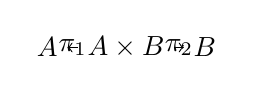
\begin{tikzpicture}
  \node (A)  {$A$};
  \node (AB) [right of=A] {$A \times B$};
  \node (B) [right of=AB] {$B$};
  \path[->]
    (AB) edge node [swap] {$\pi_1$} (A)
         edge node {$\pi_2$} (B);
 \end{tikzpicture}
\end{center}
が存在することに注目しよう.そして実際,任意の元$c \in A \times B$につい
て次が成り立つ.
\[
 c = (\pi_1 c, \pi_2 c)
\]
この状況は,次の図式により簡潔に捉えることが出来る.
\begin{center}
 \begin{tikzpicture}
  \matrix (m) [matrix of math nodes, column sep=2cm, row sep=2cm] {
     &  1  \\
   A & A \times B & B\\
  };
  \path[->]
    (m-1-2) edge node [swap] {$a$} (m-2-1)
            edge node {$b$} (m-2-3)
    (m-2-2) edge node {$\pi_1$} (m-2-1)
    (m-2-2) edge node [swap] {$\pi_2$} (m-2-3);
  \path[->, dotted] (m-1-2) edge node {$(a,b)$} (m-2-2);
 \end{tikzpicture}
\end{center}
元を一般化元で置き換えることにより,次の定義を得る.

\begin{definition}
 任意の圏${\bf C}$において,対象$A$と$B$の{\bfseries 直積図式}
 % \index{ちよくせき@直積|textit}
 \index{ふへんしやそうせい@普遍写像性!ちよくせきの@直積の---}
 \index{すしき@図式!ちよくせき@直積---}は,対象 $P$ と射
 \begin{center}
  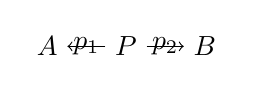
\begin{tikzpicture}
   \node (A) {$A$};
   \node (P) [right of=A]{$P$};
   \node (B) [right of=P]{$B$};
   \path[->]
     (P) edge node [swap]{$p_1$} (A)
         edge node {$p_2$} (B);
  \end{tikzpicture}
 \end{center}
 から成り,次の普遍写像性を満たす.

 次の形の図式
 \begin{center}
  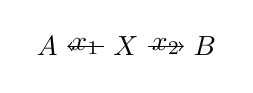
\begin{tikzpicture}
   \node (A) {$A$};
   \node (X) [right of=A]{$X$};
   \node (B) [right of=X]{$B$};
   \path[->]
     (X) edge node [swap]{$x_1$} (A)
         edge node {$x_2$} (B);   
  \end{tikzpicture}
 \end{center}
 が与えられた時,次の図式を可換にする$u: X \to P$が一意的に存在する.
 \begin{center}
  \begin{tikzpicture}
   \matrix (m) [matrix of math nodes, column sep=2cm, row sep=2cm] {
      &  X  \\
    A & A \times B & B\\
   };
   \path[->]
    (m-1-2) edge node [swap] {$x_1$} (m-2-1)
            edge node {$x_2$} (m-2-3)
    (m-2-2) edge node {$p_1$} (m-2-1)
    (m-2-2) edge node [swap] {$p_2$} (m-2-3);
   \path[->, dotted] (m-1-2) edge node {$u$} (m-2-2);
  \end{tikzpicture}
 \end{center}
 すなわち,$x_1 = p_1 u,\, x_2 = p_2 u$を満たす.
\end{definition}
\index{けん@元!いつはんか@一般化---|)}
\begin{remark}
 他の普遍写像性と同様,この定義は二つの部分からなっている.
 \begin{description}
  \item[存在:] $x_1 = p_1 u,\,x_2 = p_2 u$を満たすある$u: X \to U$が存
	     在する.
  \item[一意性:] 任意の$v: X \to U$について,$p_1 v = x_1,\,p_2 v =
	     x_2$ならば$v = u$である.
 \end{description}
\end{remark}

\begin{prop}
 直積は同型を除いて一意である.
\end{prop}
\begin{proof}
 二つの$A$と$B$の直積
 \begin{center}
  \begin{tikzpicture}
   \matrix (m) [matrix of math nodes, column sep=2cm, row sep=0.5cm] {
    A & P & B\\
    A & Q & B\\
   };
   \path[->]
     (m-1-2) edge node [swap]{$p_1$} (m-1-1)
             edge node {$p_2$} (m-1-3)
     (m-2-2) edge node [swap]{$q_1$} (m-2-1)
             edge node {$q_2$} (m-2-3);   
  \end{tikzpicture}
 \end{center}
 があったとしよう.この時,$Q$は直積であるので,$i:P \to Q$が一意に存在
 して,$q_1\circ i = p_1$かつ$q_2\circ i = p_2$を満たす.同様に$P$が直積
 であることから,一意な射$j: Q \to P$が存在し,$p_1\circ j = q_1$かつ
 $p_2\circ j = q_2$を満たす.

 \begin{center}
  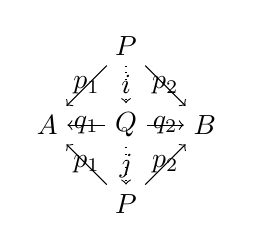
\begin{tikzpicture}
   \node (Q)  {$Q$};
   \node (P1) [above of=Q] {$P$};
   \node (P2) [below of=Q] {$P$};
   \node (A)  [left of=Q]  {$A$};
   \node (B)  [right of=Q] {$B$};

   \path[->]
     (Q)  edge node {$q_1$} (A)
          edge node [swap] {$q_2$} (B)
     (P1) edge node [swap] {$p_1$} (A)
          edge node {$p_2$} (B)
     (P2) edge node {$p_1$} (A)
          edge node [swap] {$p_2$} (B);
   \path[->, dotted]
     (P1) edge node {$i$} (Q)
     (Q)  edge node {$j$} (P2);
  \end{tikzpicture}
 \end{center}
 合成すると,$p_1 \circ j \circ i = p_1,\, p_2 \circ j \circ i = p_2$とな
 る.ここで,$p_1 \circ 1_P = p_1,\, p_2 \circ 1_P = p_2$ も成立している
 ので,射の一意性の条件より$j \circ i = 1_P$となり,同様にして,$i \circ
 j = 1_Q$を得る.従って,$i: P \to Q$は同型射となる.
\end{proof}
$A$と$B$が直積を持つとき,そのうちの一つを
\begin{center}
 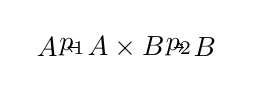
\begin{tikzpicture}
   \node (A) {$A$};
   \node (P) [right of=A]{$A\times B$};
   \node (B) [right of=P]{$B$};
   \path[->]
     (P) edge node [swap]{$p_1$} (A)
         edge node {$p_2$} (B);
 \end{tikzpicture}
\end{center}
と書く.ここで,定義の$X,x_1,x_2$が与えられたとき,
\[
 \langle x_1, x_2 \rangle \text{で} u: X \to A \times B
\]
を表わす.

しかし,注意すべきなのは,対象の組は圏の中で複数の異なる直積を持ちうる,
ということである.例を挙げれば,直積$A \times B, p_1, p_2$とある同型射
$i: A \times B \to Q$が与えられたとき,図式
$Q, p_1 \circ h, p_2 \circ h$もまた$A$と$B$の直積となる.

さて,直積{\bfseries への}射
\[
 f: X \to A \times B
\]
は射の組
\[
 f_1: X \to A,\ \ \ f_2: X \to B
\]
と「同じもの」なのであった.したがって,そうした射のことは本質的に忘れて
しまっても問題がない.なぜなら,そういった射は射の組によって一意的に決定
されるからである.しかし,圏が積をもつとき,ある有用な概念を得ることが
{\bfseries できる}.つまり,直積{\bfseries からの}射
\[
 g: A \times B \to Y
\]
を考えることが出来る.このような$g$は「2変数函数」である.つまり,任意の
二つの一般化元$f_1: X \to A,\, f_2:X \to B$が与えられたとき,元
$g\langle f_1, f_2 \rangle: X  \to Y$を得ることが出来る.このような射
$g: A\times B \to Y$は,射が直積へと入射する場合とは異なり,より基本的な
形には「簡約可能(reducible)」ではない(念の為にいえば,これらは「カリー化」
$\lambda f : A \to Y^B$を通じて「冪」$Y^B$と関連している.詳細は第
\ref{Ch:exponentials}章で扱う).
\section{直積の例}
\label{直積の例}
\begin{enumerate}
 \item 集合のデカルト積は既に扱った.順序対 $\langle a,b \rangle$に異な
       る定義を採用した場合,それぞれに対応する異なる集合
       \[
	A \times B\ \ \text{と}\ \  A \times ' B
       \]
       を考えることが出来る.これらは共に直積(の一つ)であり,それぞれ
       同型となる.例えば,異なる定義の例として,以下のように取ることが
       出来る.
       \begin{align*}
	\langle a, b\rangle &= \{\{a\}, \{a, b\}\}\\
	\langle a, b\rangle ' &= \langle \langle a\rangle, \langle a, b\rangle\rangle
       \end{align*}
       
 \item モノイドや群のような「構造の入った集合」の直積は,しばしばその台
       集合の直積に{\bfseries 成分ごと}の演算を入れたものとして構成する
       ことが出来る.例えば,$G, H$が群のとき,$G\times H$は台集合を
       $\Set{\langle g, h\rangle | g \in G, h \in H}$として,二項演算を,
       \[
	\langle g, h \rangle \cdot \langle g', h'\rangle
         = \langle g \cdot g', h \cdot h' \rangle
       \]
       単位元を
       \[
	u = \langle u_G, u_H \rangle
       \]
       逆元を
       \[
	\langle g, h \rangle^{-1} = \langle g^{-1}, h^{-1} \rangle
       \]
       で定めたものとして構成できる.射影準同型
       $G \times H \to G\ (\text{or}\ H)$は明らかに
       $\langle g, h\rangle \mapsto g\ (\text{or}\ h)$ である.
 \item 同様に,${\bf C}, {\bf D}$が圏のとき,対象および射の組から成る圏
       \[
	{\bf C} \times {\bf D}
       \]
       も既に定義してあった.自明な射影函手と合わせれば,(もし${\bf C},
       {\bf D}$が小さければ)これは実際$\Cat$ での直積となる.(このことを
       確かめよ.つまり,こうして定義された直積圏が直積の普遍写像性を満
       たすことを示せ.)

       より特別な場合として,poset の直積およびモノイドの直積を,それぞ
       れを圏と見做したときの直積として得ることが出来る.(確認:射影も
       写像の組から一意に得られる射も単調写像となること,また$\Cat$にお
       いて構成されたposetの直積が$\Pos$においても直積となっていること
       を示せ.$\Mon$の場合も同様の考察を行え.)
 \item $P$ を poset として元$p, q \in P$の直積を考えよう.この時,射影
       \begin{align*}
	p \times q &\leq p\\
	p \times q &\leq q
       \end{align*}
       が存在しなくてはならない.また,任意の元$x$に対して,
       \[
	x \leq p\ \text{かつ}\ x \leq q
       \]
       が成立するなら,
       \[
	x \leq p \times q
       \]
       でなくてはならない.

       この演算$p\times q$が何であるかわかるだろうか?それはいわゆる
       {\bfseries 下限}$p\times q = p \wedge q$である.後程見てゆくよう
       に,他の順序論的概念も圏論の概念の特別な場合であることが多い.
 \item (位相空間について幾らか知っている人向けの例.)二つの{\bfseries 位相
       空間}$X, Y$の通常の定義による直積空間が,位相空間と連続写像の圏
       ${\bf Top}$で実際に直積となることを示そう.そこで,位相空間$X,Y$
       とその直積空間$X \times Y$および射影
       \begin{center}
	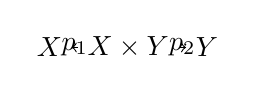
\begin{tikzpicture}
	 \node (X) {$X$};
	 \node (XxY) [right of=X] {$X \times Y$};
	 \node (Y) [right of=XxY] {$Y$};

	 \path [->]
	   (XxY) edge node {$p_2$} (Y)
	         edge node [swap] {$p_1$} (X);
	\end{tikzpicture}
       \end{center}
       が与えられているとしよう.$O(X \times Y)$
       \footnote{訳注:ここでは空間 $S$ の開集合系を $O(S)$ で表わしてい
       る.}は, $U\in O(X), V \in O(Y)$に対して$U \times V$の形の集合を
       開基として生成されることを思い出そう.つまり,任意の$W \in O(X\in
       Y)$ はそのような開基の和集合として表わすことが出来る.

       \begin{itemize}
	\item $p^{-1}U = U \times Y$ より明らかに $p_1$ は連続.
	      \footnote{訳注:標準射影$p_1, p_2$を共に連続とする位相の中
	      で最も弱いものとして積位相を定義することもある.その場合,
	      ここの議論は自明となる.}
	\item 連続写像$f_1: Z \to X, f_2: Z \to Y$ が与えられたとき,写
	      像$f: Z \to X \times Y$を $f = \langle f_1, f_2
	      \rangle$によって定める.あとは, $f$が連続であることを示せ
	      ば良い.
	\item 任意の $W = \bigcup_{i} (U_i \times V_i) \in O(X \times
	      Y)$に対し,$f^{-1}(W) = \bigcup_{i} f^{-1}(U_i \times
	      V_i)$が成立する.よって,あとは $f^{-1}(U \times V)$が開集
	      合となることを示せばよい.ところで,
	      \begin{align*}
	       f^{-1}(U \times V)
	       &= f^{-1}((U \times Y) \cap (X \times V))\\
	       &= f^{-1}(U \times Y) \cap f^{-1}(X \times V)\\
	       &= f^{-1} \circ p_1^{-1}(U) \cap f^{-1} \circ
	          p_2^{-1}(V)\\
	       &= (f_1)^{-1}(U) \cap (f_2)^{-1}(V)
	      \end{align*}
	      であり,また$f_1, f_2$は連続よりその逆像$(f_1)^{-1}(U),
	      (f_2)^{-1}(V)$は共に開集合となる.よって示された.

	      次の図式はこの状況を端的かつ簡潔に捉えたものとなっている.
	      \begin{center}
	       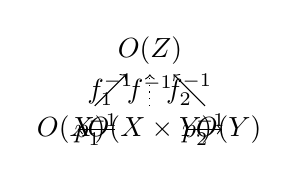
\begin{tikzpicture}
		\node (Z) {$O(Z)$};
		\node (XY) [below of=Z] {$O(X\times Y)$};
		\node (X) [left of=XY] {$O(X)$};
		\node (Y) [right of=XY] {$O(Y)$};

		\path[->]
		  (X) edge node {$f_1^{-1}$} (Z)
		      edge node [swap]{$p_1^{-1}$} (XY)
		  (Y) edge node [swap]{$f_2^{-1}$} (Z)
		      edge node {$p_2^{-1}$} (XY);
		\path[->, dotted] (XY) edge node [swap] {$f^{-1}$} (Z);
	       \end{tikzpicture}
	      \end{center}
       \end{itemize}
 \item (型理論に馴染みのある人向けの例.)(単純型付き)$\lambda$計算の
      について考えよう.$\lambda$計算とは,「変数束縛」
       と函数の評価に基づいた,函数概念の明確化と操作のための形式系であ
       る.例として,実係数多項式$x^2 + 2y$を考えよう.$\lambda$計算では,
       (各固定値$x$に対する)函数$y \mapsto x^2 + 2y$を
       $\lambda y. x^2 + 2y$と書き,函数$x \mapsto (y \mapsto x^2 + 2y)$
       を表わすのに$\lambda x. \lambda y. x^2 + 2y$と書く.

       形式的には,$\lambda$計算は次の要素から成る.
       \label{型の圏}
       \begin{itemize}
	\item 型:$A \times B, A \to B, \ldots$(幾つかの基本型から生成
	      される)
	\item 項:
	      \begin{align*}
	       x, y, z,\ldots : A   \ &\ \text{(各型$A$に対する変数)}\\
	       a:A, b:B,\ldots : A  \ &\ \text{(ありうる幾つかの型付き定数)}\\
	       \langle a, b \rangle: A \times B \ &\ (a: A, b: B)\\
	       \mathrm{fst}(c): A   \ &\ (c: A \times B)\\
	       \mathrm{snd}(c): B   \ &\ (c: A \times B)\\
	       ca : B               \ &\ (c: A \to B, a : A)\\
	       \lambda x.b: A \to B \ &\ (x: A, b: B)
	      \end{align*}
	\item 等式:
	      \begin{align*}
	       \mathrm{fst}(\langle a, b \rangle) &= a\\
	       \mathrm{snd}(\langle a, b \rangle) &= b\\
	       \langle \mathrm{fst}(c), \mathrm{snd}(c) \rangle
	         &= c\\
	       (\lambda x. b)a &= b[a/x]\\
	       \lambda x. cx &= c\ \ \text{($x$ が $c$ に現れない場合)}
	      \end{align*}
       \end{itemize}

       項の二項関係$a \sim b$(通常{\bfseries $\beta\eta$-同値性}と呼ば
       れる)は,上の等式から生成される同値関係に,束縛変数の付け替え
       \[
       \lambda x. b = \lambda y. b[y/x]
       \ \ \text{($b$に$y$が現れない場合)}
       \]
       を付け加えたものである.
       
       そこで,型の圏${\bf C}(\lambda)$は次のように定義される:
       \begin{itemize}
	\item 対象:型
	\item 射$A \to B$:閉じた項 $c: A \to B$を同値関係
	      $c \sim c'$によって同一視したもの.
	\item 恒等射:$1_A = \lambda x. x\ \ (\text{ただし}x: A)$
	\item 合成射:$c \circ b = \lambda x. c(bx)$
       \end{itemize}
       この圏がwell-definedであることを見よう.\\
       単位律:
       \begin{align*}
	c \circ 1_B &= \lambda x(c((\lambda y.y)x)) = \lambda x(cx) = c\\
	1_A \circ c &= \lambda x((\lambda y.y)(cx)) = \lambda x(cx) = c
       \end{align*}
       結合律:
       \begin{align*}
	c \circ (b \circ a)
	&= \lambda x(c((b \circ a) x))\\
	&= \lambda x(c((\lambda y. b(ay)) x))\\
	&= \lambda x(c(b(ax)))\\
	&= \lambda x(\lambda y(c(by))(ax))\\
	&= \lambda x((c \circ b)(ax))\\
	&= (c \circ b) \circ a
       \end{align*}
       この圏は二項直積を持つ.実際,型$A, B$が与えられているとし,
       \[
        p_1 = \lambda z. \mathrm{fst}(z),\,\,
        p_2 = \lambda z. \mathrm{snd}(z)\ \ (z: A \times B)
       \]
       としよう.そして下図のような$a, b$が与えられているとする.
       \begin{center}
	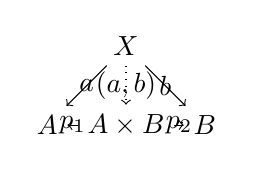
\begin{tikzpicture}
	 \node (X)  {$X$};
	 \node (AxB)[below of=X] {$A \times B$};
	 \node (A) [left of=AxB] {$A$};
	 \node (B) [right of=AxB]{$B$};

	 \path[->]
	   (X) edge node [swap]{$a$} (A)
	       edge node {$b$} (B)
	   (AxB) edge node {$p_1$} (A)
	         edge node [swap]{$p_2$} (B);
	 \draw[->, dotted] (X) to node {$(a, b)$} (AxB);
	\end{tikzpicture}
       \end{center}
       但し
       \[
	(a, b) = \lambda x. \langle ax, bx \rangle
       \]
       である.すると,
       \begin{align*}
	p_1 \circ (a, b)
	&= \lambda x(p_1((\lambda y.\langle ay, by\rangle)x))\\
	&= \lambda x(p_1 \langle ax, bx \rangle)\\
	&= \lambda x(ax)\\
	&= a
       \end{align*}
       であり,同様に$p_2 \circ (a, b) = b$となる.

       最後に$c: X \to A \times B$とすると
       \[
	p_1 \circ c = a,\,\,p_2 \circ c = b
       \]
       がありこの時,
       \begin{align*}
	(a, b)
	&= \lambda x. \langle ax, bx \rangle\\
	&= \lambda x. \langle (p_1 \circ c)x, (p_2 \circ c)x \rangle\\
	&= \lambda x. \langle (\lambda y(p_1(cy)))x,
	               (\lambda y(p_2(cy)))x \rangle\\
	&= \lambda x. \langle (\lambda y((\lambda z.\mathrm{fst}(z))(cy)))x,
	            (\lambda y((\lambda z.\mathrm{snd}(z))(cy)))x \rangle\\
	&= \lambda x. \langle \lambda y(\mathrm{fst}(cy))x,
	            \lambda y(\mathrm{snd}(cy))x \rangle\\
	&= \lambda x. \langle \mathrm{fst}(cx), \mathrm{snd}(cx) \rangle\\
	&= \lambda x. cx\\
	&= c
       \end{align*}
       となる.
\end{enumerate}
\begin{remark}\label{Curry-Howard}
 $\lambda$計算にはもう一つ驚くべき解釈がある.すなわち,命題計算における
 証明概念の体系として解釈出来るのである.この対応は「Curry-Howard」対応
 として知られている.手短かにいえば,型を命題($A \times B$を連言(論理
 積),$A \to B$ を含意)として解釈し,項$a: A$を命題$A$の証明と考えるの
 である.以下のような形の項の形成規則
 \begin{prooftree}
  \AxiomC {$a: A$} \AxiomC{$b: B$}
  \BinaryInfC{$\langle a, b \rangle : A \times B$}
 \end{prooftree}
 は,証明のラベルを帰納的に組み上げる方法を示した注釈付きの推論規則とし
 て読むことが出来る.そこで例えば,前提のキャンセルを角括弧で表わすことに
 すると,
 \begin{prooftree}
  \AxiomC{$[A]$} \AxiomC{$[B]$}
  \BinaryInfC{$A \times B$}
  \UnaryInfC{$B \to (A \times B)$}
  \UnaryInfC{$A \to (B \to (A \times B))$}
 \end{prooftree}
 のような自然演繹の証明は,次のようにラベル付けすることが出来る.
 \begin{prooftree}
  \AxiomC{$[x: A]$} \AxiomC{$[y: B]$}
  \BinaryInfC{$\langle x, y \rangle :A \times B$}
  \UnaryInfC{$\lambda y.\langle x, y \rangle : B \to (A \times B)$}
  \UnaryInfC{$\lambda x \lambda y. \langle x, y \rangle :A \to (B \to (A
  \times B))$}
 \end{prooftree}
 従って,最後の「証明項」$\lambda x\lambda y. \langle x, y \rangle$は
 「命題」$A \to (B \to (A \times B))$の証明の筋道を記録しており,同じ命
 題に対する異なる証明は異なる項を与えることがある.

 結果として得られる論理と型理論の「同型」について言及されることがしばし
 ばあるが,ここで我々が実際に扱っているのは,単に(
 \ref{Sec:Example of Categories}節の例\ref{example of logic}で定義した)
 連言と含意を持つ命題計算の圏から$\lambda$計算の圏への函手にすぎない.一
 般的に,証明の間に更に何らかの等式をおかない限り,この函手は同型射には
 ならない.
\end{remark}
\section{直積のある圏}
${\bf C}$を,任意の対象の組が直積図式を持つ圏とする.下図のような直積を
持った対象と射があったとしよう.
\begin{center}
 \begin{tikzpicture}
  \matrix (m) [matrix of math nodes, column sep=2cm, row sep=2cm] {
  A & A \times A' & A'\\
  B & B \times B' & B'\\
  };

  \path[->]
    (m-1-1) edge node [swap] {$f$} (m-2-1)
    (m-1-2) edge node [swap] {$p_1$} (m-1-1)
            edge node {$p_2$} (m-1-3)
    (m-1-3) edge node {$f'$} (m-2-3)
    (m-2-2) edge node {$q_1$} (m-2-1)
            edge node [swap]{$q_2$} (m-2-3);
 \end{tikzpicture}
\end{center}
このとき,$f \times f' = \langle f \circ p_1, f' \circ p_2 \rangle$ によっ
て
\[
 f \times f' : A \times A' \to B \times B'
\]
を定める.従って,下の図式の二つの長方形は可換となる.
\begin{center}
 \begin{tikzpicture}
  \matrix (m) [matrix of math nodes, column sep=2cm, row sep=2cm] {
  A & A \times A' & A'\\
  B & B \times B' & B'\\
  };

  \path[->]
    (m-1-1) edge node [swap] {$f$} (m-2-1)
    (m-1-2) edge node [swap] {$p_1$} (m-1-1)
            edge node {$p_2$} (m-1-3)
    (m-1-3) edge node {$f'$} (m-2-3)
    (m-2-2) edge node {$q_1$} (m-2-1)
            edge node [swap]{$q_2$} (m-2-3);
  \draw[->, dotted] (m-1-2) to node {$f \times f'$}(m-2-2);
 \end{tikzpicture}
\end{center}
こうして,任意の二つの対象に対しその直積を選んでやることで,函手
\[
 \times : {\bf C} \times {\bf C} \to {\bf C}
\]
を得る.これが函手となることは,直積の普遍写像性を使うことによって読者が
簡単に確かめられるだろう.ある圏が任意の二つの対象に対する直積を持つとき,
その圏は{\bfseries 二項直積を持つ}という.

似たような普遍写像性によって三項直積
\[
 A_1 \times A_2 \times A_3
\]
も定義することが出来る(三つの射影$p_i: A_1 \times A_2 \times A_3 \to
A_i$があって,任意の対象 $X$と三つの射$x_i: X \to A_i$に対し射
$u: X \to A_1 \times A_2 \times A_3$が一意に存在して,$p_i u = x_i$を満
たす).このような条件は明らかに任意個の因子に対して考えることが出来る.

一方で,もし圏が二項直積を持てば,明らかに二つ以上の因子からなる任意の有
限直積を持つ.例えば,
\[
 A \times B \times C = (A \times B) \times C
\]
とすれば三項直積の普遍写像性は満たされる.他方,$A\times (B\times C)$を
定義として採用してもよい.この事実は,二項直積$A\times B$は同型を無視す
れば結合律を満たすということを意味する.何故なら三項直積の普遍写像性より,
\[
 (A \times B) \times C \cong A \times (B \times C)
\]
が成立しなくてはならないからである.

終対象が「無項」直積(nullary product)となっていることに注目しよう:
\begin{quotation}
 ゼロ個の対象が与えられた時,ゼロ個の射影を持つ対象$1$があり,他の対象
 $X$とゼロ個の射が与えられれば,射
 \[
  ! : X \to 1
 \]
 が一意に存在して,特にどんな図式も可換にしない.
\end{quotation}
同様に,任意の対象$A$はそれ自身を一度だけ乗じた,$A$の{\bfseries 単項直
積}({\itshape unary product})である.

最後に,{\bfseries 任意の}集合$I$で添字付けられた対象の族
$(C_i)_{i \in I}$の直積を,無項,単項,二項,$n$項直積からの類推によって
「$I$項直積」の普遍写像性を与えることで定義することが出来る.この精確な
定式化は演習問題とする.

\begin{definition}
 圏${\bf C}$が{\bfseries 任意の有限直積を持つ}とは,終対象と任意の二項直
 積を持つ(従って任意の有限濃度の直積を持つ)ことである.圏${\bf C}$が
 {\bfseries 任意の(小さな)直積を持つ}とは,${\bf C}$の対象から成る任意
 の集合が直積を持つことである.
\end{definition}
\index{ちよくせき@直積|)}
\section{$\Hom$集合}
この節では,局所的に小さな圏のみを考えよう.

任意の圏${\bf C}$について,対象$A, B$が与えらえたとき,
\[
 \Hom(A, B) = \Set{f \in {\bf C} | f: A \to B}
\]
と書き,このような射の集合を {\itshape Hom}{\bfseries 集合}と呼んだこと
を思い出そう.${\bf C}$の任意の射 $g: B \to B'$は写像
\begin{align*}
 \Hom(A, g): \Hom(A, B) \to \Hom(A, B')\\
 (f: A \to B) \mapsto (g \circ f : A \to B \to B')
\end{align*}
を引き起こすことに注意する.つまり,$\Hom(A, g) = g \circ f$である
\footnote{訳注:正しくは$\Hom(A, g)(f) = g \circ f$と書くべき?}.
$\Hom(A, g)$の代わりに$g_{\ast}$と書くこともある.つまり,
\[
 g_{\ast}(f) = g \circ f
\]
である.

これが$A$の(共変){\bfseries 表現可能函手}({\itshape representable
functor})と呼ばれる函手
\[
 \Hom(A, -): {\bf C} \to \Sets
\]
を定めることを示そう.我々が示すべきことは,
\[
 \Hom(A, 1_{X}) = 1_{\Hom(A, X)}
\]
と
\[
 \Hom(A, g \circ f) = \Hom(A, g) \circ \Hom(A, f)
\]
の二つである.引数$x: A \to X$を取れば明らかに,
\begin{align*}
 \Hom(A, 1_X)(x) &= 1_X \circ x\\
                 &= x\\
                 &= 1_{\Hom(A, X)}(x)
\end{align*}
であり,
\begin{align*}
 \Hom(A, g \circ f)(x) &= (g \circ f) \circ x\\
                       &= g \circ (f \circ x)\\
                       &= \Hom(A, g)(\Hom(A, f)(x))
\end{align*}
となる.

こうした表現可能函手については後程より慎重に学んでゆく.目下のところは,
もうひとつの直積の定義の定式化を得るのにHom集合をどのように用いることが
出来るかを見ていきたい.

任意の対象 $P$ に対して,二つの射$p_1: P \to A$および $p_2: P \to B$は集
合
\[
 \Hom(P, A) \times \Hom(P, B)
\]
の元$(p_1, p_2)$を決定する.さて,任意の射
\[
 x: X \to P
\]
が与えられたとき,その$p_1$および$p_2$との合成は,下図に示すような二つの
射$x_1 = p_1 \circ x: X \to A$ および $x_2 = p_2 \circ x: X \to B$を与え
る.
\begin{center}
 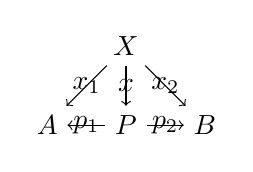
\begin{tikzpicture}
  \node (X) {$X$};
  \node (P) [below of=X] {$P$};
  \node (A) [left of=P] {$A$};
  \node (B) [right of=P] {$B$};
  \path[->]
    (X) edge node [swap]{$x_1$} (A)
        edge node {$x$} (P)
        edge node {$x_2$} (B)
    (P) edge node {$p_1$} (A)
        edge node [swap] {$p_2$} (B);
 \end{tikzpicture}
\end{center}
このようにして,
\begin{equation}
  \vartheta_X(x) = (x_1, x_2)\label{phi_X}
\end{equation}
で定義される写像
\[
 \vartheta_X = (\Hom(X, p_1), \Hom(X, p_2))
           : \Hom(X, P) \to \Hom(X, A) \times \Hom(X, B)
\]
を得る.この写像$\vartheta_X$により,直積であるための条件を次のように簡潔
に表現することが出来る.
\begin{prop}\label{Homs and products}
 図式
 \begin{center}
  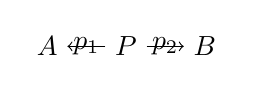
\begin{tikzpicture}
   \node (P) {$P$};
   \node (A) [left of=P] {$A$};
   \node (B) [right of=P] {$B$};

   \path[->]
     (P) edge node {$p_1$} (A)
         edge node [swap]{$p_2$} (B);
  \end{tikzpicture}
 \end{center}
 が$A$と$B$の直積であるための必要十分条件は,$(\ref{phi_X})$で与えられる自
 然な写像$\vartheta_X$が同型
 \[
  \vartheta_X: \Hom(X, P) \cong \Hom(X, A) \times \Hom(X, B)
 \]
 となっていることである.
\end{prop}
\begin{proof}
 直積の普遍写像性を確かめよう.普遍写像性の主張はまさに任意の元
 $(x_1, x_2) \in \Hom(X, A) \times \Hom(X, B)$に対し,
 $x \in \Hom(X, P)$が一意に存在し,$\vartheta_X(x) = (x_1, x_2)$となるとい
 うことである.従って$\vartheta_X$は全単射となる.
\end{proof}

\begin{definition}
 ${\bf C}, {\bf D}$を二項直積を持つ圏とする.函手$F: {\bf C} \to {\bf
 D}$が{\bfseries 二項直積を保存する}とは,$F$が${\bf C}$の任意の直積図式
 \begin{center}
  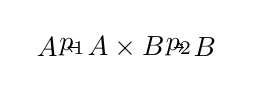
\begin{tikzpicture}
   \node (P) {$A \times B$};
   \node (A) [left of=P] {$A$};
   \node (B) [right of=P] {$B$};

   \path[->]
     (P) edge node {$p_1$} (A)
         edge node [swap]{$p_2$} (B);
  \end{tikzpicture}
 \end{center}
 を${\bf D}$の直積図式
  \begin{center}
  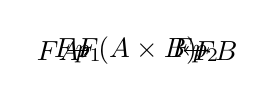
\begin{tikzpicture}
   \node (P) {$F(A \times B)$};
   \node (A) [left of=P] {$FA$};
   \node (B) [right of=P] {$FB$};

   \path[->]
     (P) edge node {$Fp_1$} (A)
         edge node [swap]{$Fp_2$} (B);
  \end{tikzpicture}
 \end{center}
 に移すことである.
\end{definition}
$F$が直積を保存するのは,
\[
 F(A \times B) \cong FA \times FB
\]
が「標準的な(canonical)」同型であるときのみであることがわかる.つまり,
${\bf D}$の標準的な「比較射」
\[
 \langle Fp_1, Fp_2\rangle : F(A \times B) \to FA \times FB
\]
が同型射であるとき,その時に限って$F$は直積を保存する.

例えば,忘却函手$U: \Mon \to \Sets$は二項直積を保存する.

\begin{corollary}
 ${\bf C}$を直積を持つ圏とする.任意の${\bf C}$の対象$X$に対し,(共変)
 表現可能函手
 \[
  \Hom_{\bf C}(X, -): {\bf C} \to \Sets
 \]
 は直積を保つ函手である.
\end{corollary}
\begin{proof}
 任意の$A, B \in {\bf C}$に対し,上の命題\ref{Homs and products}によって
 標準的な同型
 \[
  \Hom_{\bf C}(X, A \times B)
   \cong \Hom_{\bf C}(X, A) \times \Hom_{\bf C}(X, B)
 \]
 が存在することがわかる.
\end{proof}
\section{演習問題}
\begin{enumerate}
 \item 集合の間の写像は,全射である時,その時に限ってエピ射となることを
       示せ.また,$\Sets$での同型射はモニックかつエピックな射と一致する
       ことを結論せよ.
 \item 任意の poset圏において,全ての射はモニックかつエピックとなること
       を示せ.
 \item (逆射の一意性.)もし射$f: A \to B$が逆射$g, g': B \to A$を持て
       ば(つまり$g \circ f = 1_A, f \circ g = 1_B$ であり,$g'$について
       も同様とするとき),$g = g'$となることを示せ.
 \item 任意の圏${\bf C}$における可換図式
       \begin{center}
	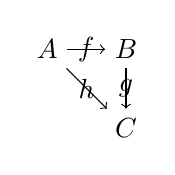
\begin{tikzpicture}
	 \node (A) {$A$}; \node (B) [right of=A] {$B$};
	 \node (C) [below of=B] {$C$};
	 \path[->]
	   (A) edge node {$f$} (B)
	       edge node [swap] {$h$} (C)
	   (B) edge node {$g$} (C);
	\end{tikzpicture}
       \end{center}
       について,次を示せ.
       \begin{enumerate}
	\item もし$f, g$が同型射(あるいはモノ射,エピ射)の時,
	      $h$も同型射(それぞれモノ射,エピ射)となる.
	\item $h$ がモニックなら $f$ もモニック.
	\item $h$ がエピックなら $g$ もエピック.
	\item $h$ がモニックであっても$g$がモニックである必要はない(例
	      を挙げよ).
       \end{enumerate}
 \item 任意の圏の射
       \[
	f: A \to B
       \]
       について,以下はすべて同値であることを示せ.
       \begin{enumerate}
	\item $f$ は同型射.
	\item $f$ はモノ射かつ分裂エピ射.
	\item $f$ は分裂モノ射かつエピ射.
	\item $f$ は分裂モノ射かつ分裂エピ射.
       \end{enumerate}
 \item グラフ準同型$h: G \to H$がモニックとなるのは,辺と頂点のそれぞれ
       について単射であるときだけであることを示せ.
 \item 任意の圏において,射影的対象のレトラクトが再び射影的となることを
       示せ.
 \item 任意の集合が(選択公理の下で)射影的であることを示せ.
 \item poset の間のエピ射は(元に関して)全射であること,一元 poset
       ${\bf 1}$は射影的であることを示せ.
 \item 任意の集合は,離散 poset と見做すことにより poset の圏で射影的対
       象となる事を示せ(いままでの演習問題を用いよ).射影的でない
       poset の例をひとつ挙げよ.任意の射影的な poset は離散的であり,し
       たがって集合と同一視できることを示せ.全ての射影的な poset とその
       間の単調写像を考えることで,$\Sets$は$\Pos$の射影的対象からなる
       「充満部分圏」(と同型)であることを示せ.
 \item $A$を集合とする.このとき,$A$-モノイドを台集合への写像
       $m: A \to U(M)$を持ったモノイド$M$として定義する.
       $A$-モノイドの射$h: (M, m) \to (N, n)$は(可換三角形)
       $U(h) \circ m = n$ を満たすモノイド準同型 $h: M \to N$である.自
       明な恒等射および合成射とあわせて,これにより$A$-モノイドからなる
       圏$A\dash\Mon$を定義することが出来る.

       $A\dash\Mon$の始対象は$A$上の自由モノイド$M(A)$と同じものであることを
       示せ.(ヒント:それぞれの普遍写像性を比較せよ.)
 \item 任意のブール代数$B$について,ブール準同型$h: B \to {\bf 2}$は$B$
       のウルトラフィルターと正確に対応していることを示せ.
 \item 二項直積を持つ任意の圏において,
       \[
	A \times (B \times C) \cong (A \times B) \times C
       \]
       を直接的に示せ.
 \item \begin{enumerate}
	\item 任意の添字集合$I$について,$I$で添字付けられた圏の対象の族
	$(X_i)_{i \in I}$の積$\prod_{i\in I} X_i$を,二項直積(つまり
	      $I = 2$の場合)を一般化した普遍写像性を与えることで定義せ
	      よ.
	\item $X$ を任意の集合として,各 $i \in I$に対し$X_i = X$で定め
	      た「定数族」を考える.$\Sets$において,$f: I \to X$なる
	      写像全体からなる集合$X^I$が上の普遍写像性を持つことを示せ.
	      すなわち,
	      \[
	       X^I \cong \prod_{i \in I} X
	      \]
	      を示せ.
       \end{enumerate}
 \item 圏${\bf C}$と対象$A, B$が与えられたとする.ここで圏
       ${\bf C}_{A, B}$ を,対象を$x_1 : X \to A,\, x_2 : X \to B$なる
       $(X, x_1, x_2)$とし,射$f: (X, x_1, x_2) \to (Y, y_1, y2)$
       は $y_1 \circ f = x_1$ かつ $y_2 \circ f = x_2$ を満たす射
       $f: X \to Y$であるような圏とする.

       ${\bf C}_{A, B}$は,$A, B$が${\bf C}$で直積を持つとき,そのときに
       に限り終対象を持つことを示せ.
 \item $\lambda$計算の型の圏${\bf C}(\lambda)$において,直積函手
       $A, B \mapsto A \times B$を直接決定せよ.また,任意に固定した型
       $A$に対して,型$X$を$A \to X$に移す函手
       $A \to (-):{\bf C}(\lambda) \to {\bf C}(\lambda)$が存在することを
       示せ.
 \item 直積を持つ任意の圏${\bf C}$において,射$f: A \to B$の{\bfseries
       グラフ} をモノ射
       \[
	\Gamma(f) = \langle 1_A, f \rangle : A \mono A \times B
       \]
       で定める(これがモノ射となるのは何故か?).特に${\bf C} = \Sets$
       のとき,これが第\ref{Categories}章で定義した二項関係の圏$\Rel$へ
       の函手$\Gamma : \Sets \to \Rel$を定めることを示せ.(実際の二項関
       係$R(f) \subseteq A \times B $を得るには
       $\Gamma(f): A \mono A \times B$の像を取ればよい.)
 \item モノイドから集合への忘却函手$U: \Mon \to \Sets$が表現可能函手であ
       ることを示せ.$U$は任意の(小さな)直積を保つことを導け.
\end{enumerate}
